Before the chain reaches its asymptotic probability distribution we need to let it evolve for a number of sweeps. Figure \ref{fig:therminit} shows that
the thermalization value is reached independently of the initialization values of $E_{J}$ for a given lattice, which we initalized in four
ways:
\begin{enumerate}
  \item with random numbers between $-1$ and $1$;
  \item  with random numbers between $-5$ and $5$;
  \item setting $x_{i}=0\ \forall i$ (cold initialization);
  \item setting $x_{i}=10\ \forall i$ (hot initialization).
\end{enumerate}
\begin{figure}[htp]
  \centering
  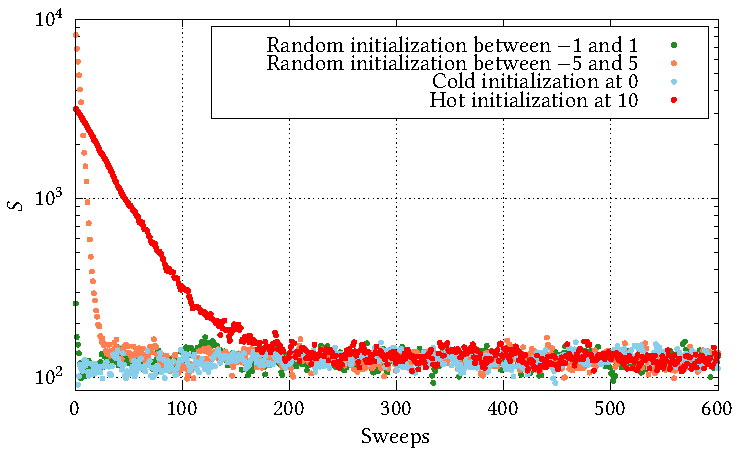
\includegraphics[width=\linewidth]{therminit}
  \caption{\label{fig:therminit} Thermalization of different Markov chains. Regardless of their initialization, they eventually start oscillating around an equilibrium value.}
\end{figure}
It is worth noting that while the thermalization value is the same, the speed is different. The \textit{colder} initialized chains take $\sim 30,50$ sweeps to thermalize, while the \textit{hot} chain needs around $\sim 200$. As a safety measure, while a colder initialization
was generally preferred,
due to the low computational costs of sweeping we decided to let each chain thermalize for $N_{therm}=1000$ sweeps\footnote{This proved to be more than enough for every lattice we considered.} throughout the whole simulation.

As we will see in subsection \ref{subsec:delta}, the width of the interval used to extract the coordinate update proposals $x_{i}'$ has an effect on the thermalization speed.

Once the chain is thermalized, it is sensible to compute the correlators.
